\documentclass[10pt]{article}
 \usepackage[margin=0.5in]{geometry} 
\usepackage{amsmath,amsthm,amssymb, graphicx, multicol, array}
  
\newenvironment{problem}[2][Problem]{\begin{trivlist}
\item[\hskip \labelsep {\bfseries #1}\hskip \labelsep {\bfseries #2.}]}{\end{trivlist}}

\begin{document}
%---------------
%---------------
 \title{Discussion - Light Interference}
\date{}
\maketitle

\begin{problem}{1}
\item
(a) 5m / 6x10-7m = 8,333,333.33 wavelengths.
\item
(b) It’s constructive, because whatever the distance to the screen may
be, it’s the same for both.
\item
(c) The amplitude goes down by a factor of two, so the intensity goes down by a factor of four.
\item
(d) Since its refractive index is between that of the middle section and that of air, both reflected rays would invert, and a path difference of $(m+1/2)\lambda$ will thus cause destructive interference in reflection.
\item
$2t = (m+1/2) \lambda/n_{coating} \longrightarrow 200nm = (m+1/2) 600nm/n_{coating}.$
\item
$n_{coating} = 3 (m+1/2)$.
\item The only possible value less than 2.25 is for m = 0, giving ncoating =
1.5.

\item
The coating will also work on the light leaving, since neither inverts. [Note: If anyone questions whether it would really prevent reflection completely, it’s probably worth mentioning that just meeting the path-length condition isn’t enough to ensure it. The other requirement--showing which is beyond the scope of the course--is that the coating’s refractive index be the square root of the substrate’s. As you can see, the numbers are chosen to work out this way.]

\item 
(e) If for the coating, 2t is half a wavelength, each holds 1/4 wavelength. The middle section holds $11,800nm / (600nm/2.25)=44.25$, giving a total in the sandwich of $44.25 + 2(.25)=44.75$. A thickness of 11,800nm + 2(100nm) = 12,000nm of air would hold 20 wavelengths of 600nm. The difference is 24.75 wavelengths. This corresponds to a phase difference of $24 \times \pi + 3\pi/2$. It’s really the “leftover” 3/4 of a cycle that is important for the intensity change.

\item
(f) The factor determining intensity is $cos^2\frac{\Delta \phi}{2}$. Whether we plug in the whole $24 \times \pi + 3\pi/2$, the answer is the same, $cos^2(3\pi/4)=0.5$. It’s down by 50\%.
\end{problem}

\begin{figure}[htp]
    \centering
    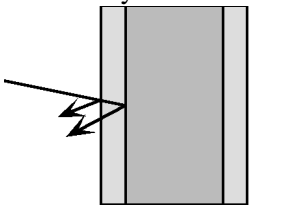
\includegraphics[width=1in]{sandwich_solution.png}
    \caption{Clear Plastic Sandwich}
    \label{fig:Graph of Wave}
\end{figure}






%-------------
%-------------
\end{document}
